\chapter{Experimental results}
After the analysis of the training and validation data, the choice fell to the TDNN, because compared to the RNN:
\begin{itemize}
	\item has got better validation accuracy and a smaller loss value;
	\item in almost every test, showed smoother training and validation curves, and was easier to train effectively.
\end{itemize}
Though, the RNN offers the benefit of learning variable-length patterns, but in this case it didn't give an advantage.
\bigbreak

Follows a comparison between the networks' testing results, based on confusion matrices, accuracy and F1 score (for the theoretical concepts see section \ref{Evaluate neural networks}).

\begin{table}[ht!]
	\centering
	\begin{tabular}{c|cccccc}
		& \textbf{Backward} & \textbf{Flight} & \textbf{Forward} & \textbf{Still} & \textbf{Thrown} & \textbf{Walking} \\ \hline
		\textbf{Backward} & 19                & 0               & 0                & 1              & 0               & 0                \\
		\rowcolor[HTML]{EFEFEF} 
		\textbf{Flight}   & 1                 & 49              & 0                & 0              & 0               & 0                \\
		\textbf{Forward}  & 0                 & 0               & 20               & 0              & 0               & 0                \\
		\rowcolor[HTML]{EFEFEF} 
		\textbf{Still}    & 0                 & 0               & 0                & 50             & 0               & 0                \\
		\textbf{Thrown}   & 0                 & 0               & 1                & 0              & 46              & 3                \\
		\rowcolor[HTML]{EFEFEF} 
		\textbf{Walking}  & 0                 & 1               & 0                & 0              & 0               & 49              
	\end{tabular}
	\caption{TDNN's confusion matrix.}
\end{table}

\begin{table}[ht!]
	\centering
	\begin{tabular}{c|cccccc}
		\textbf{}         & \textbf{Backward} & \textbf{Flight} & \textbf{Forward} & \textbf{Still} & \textbf{Thrown} & \textbf{Walking} \\ \hline
		\textbf{Backward} & 19                & 0               & 0                & 0              & 1               & 0                \\
		\rowcolor[HTML]{EFEFEF} 
		\textbf{Flight}   & 0                 & 47              & 1                & 0              & 0               & 2                \\
		\textbf{Forward}  & 0                 & 1               & 18               & 0              & 0               & 1                \\
		\rowcolor[HTML]{EFEFEF} 
		\textbf{Still}    & 0                 & 0               & 0                & 50             & 0               & 0                \\
		\textbf{Thrown}   & 0                 & 0               & 0                & 0              & 50              & 0                \\
		\rowcolor[HTML]{EFEFEF} 
		\textbf{Walking}  & 0                 & 5               & 1                & 0              & 0               & 44              
	\end{tabular}
	\caption{RNN's confusion matrix.}
\end{table}

\begin{center}
	\begin{figure}[ht!]
		\makebox[\textwidth]{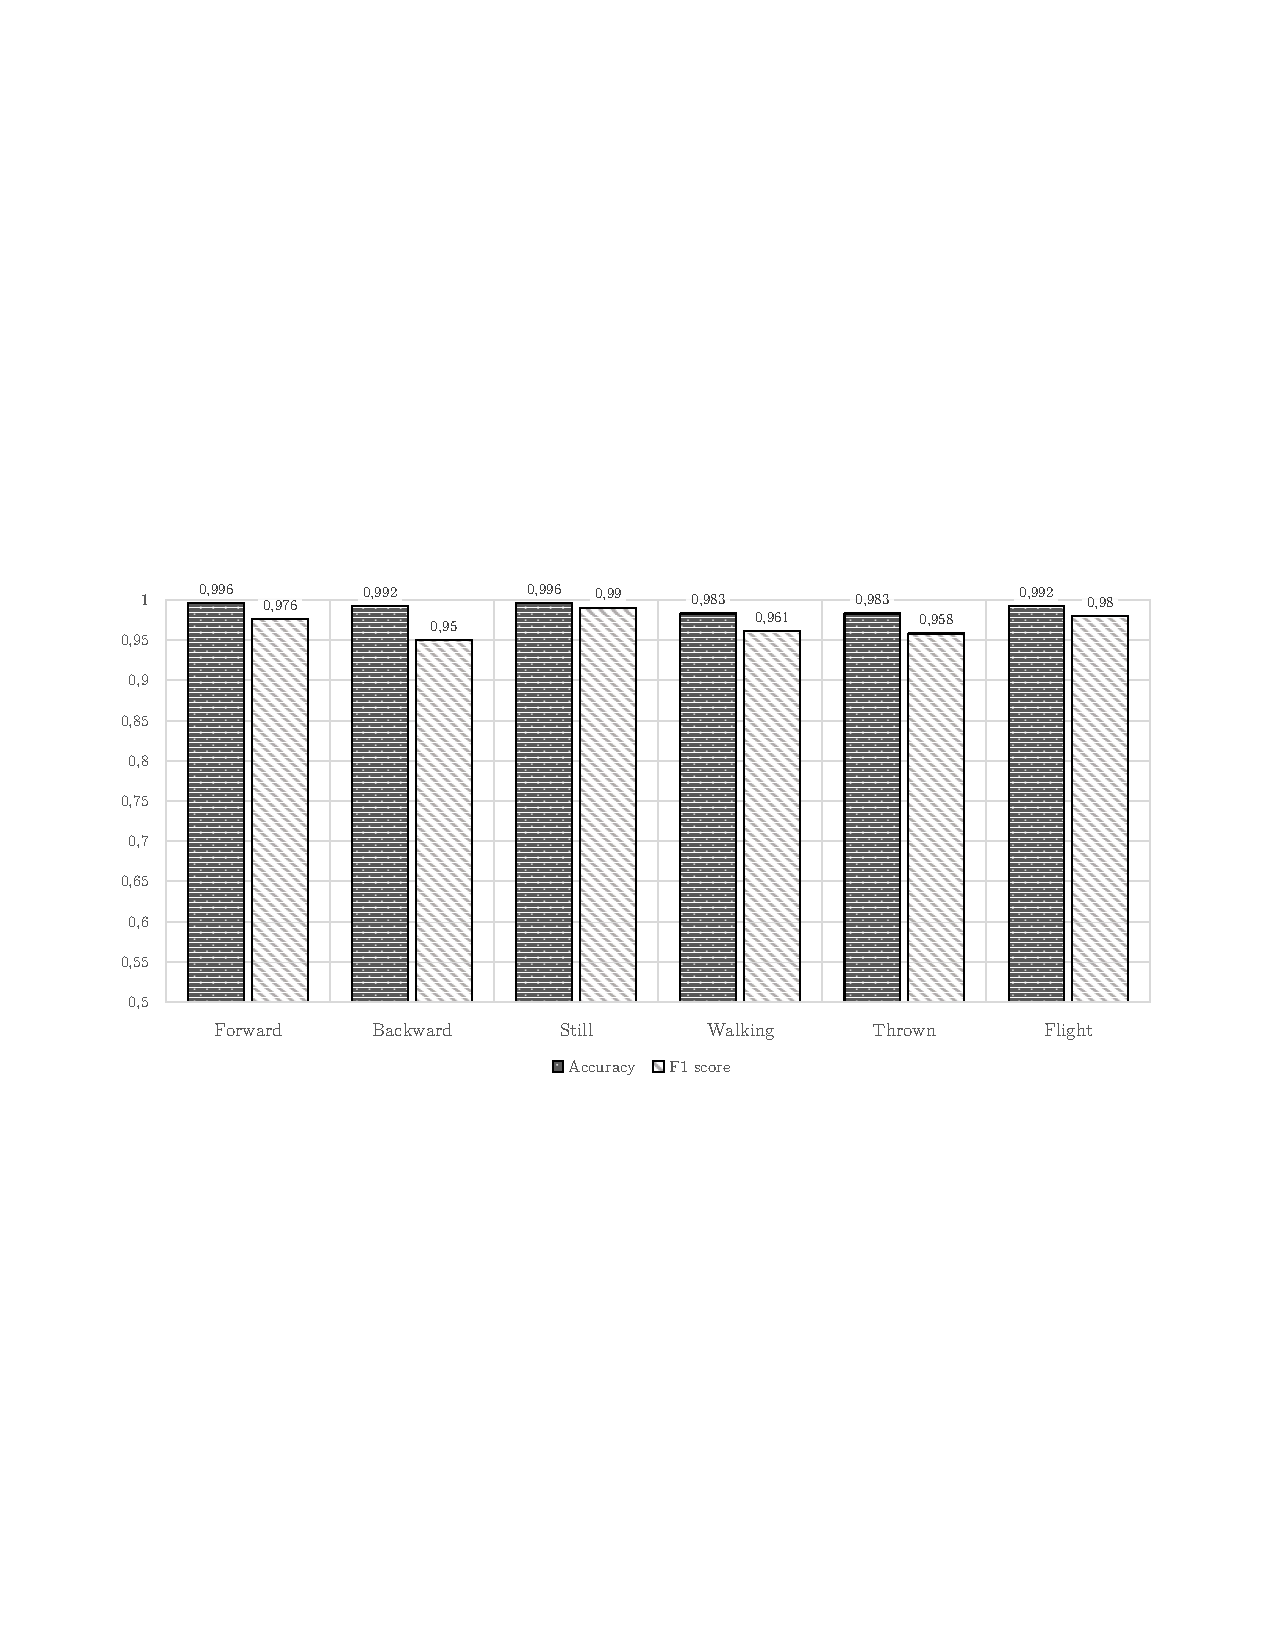
\includegraphics[width=0.8\paperwidth]{img/tdnn_results.pdf}}
		\caption{TDNN testing results.}
	\end{figure}
\end{center}

\begin{center}
	\begin{figure}[ht!]
		\makebox[\textwidth]{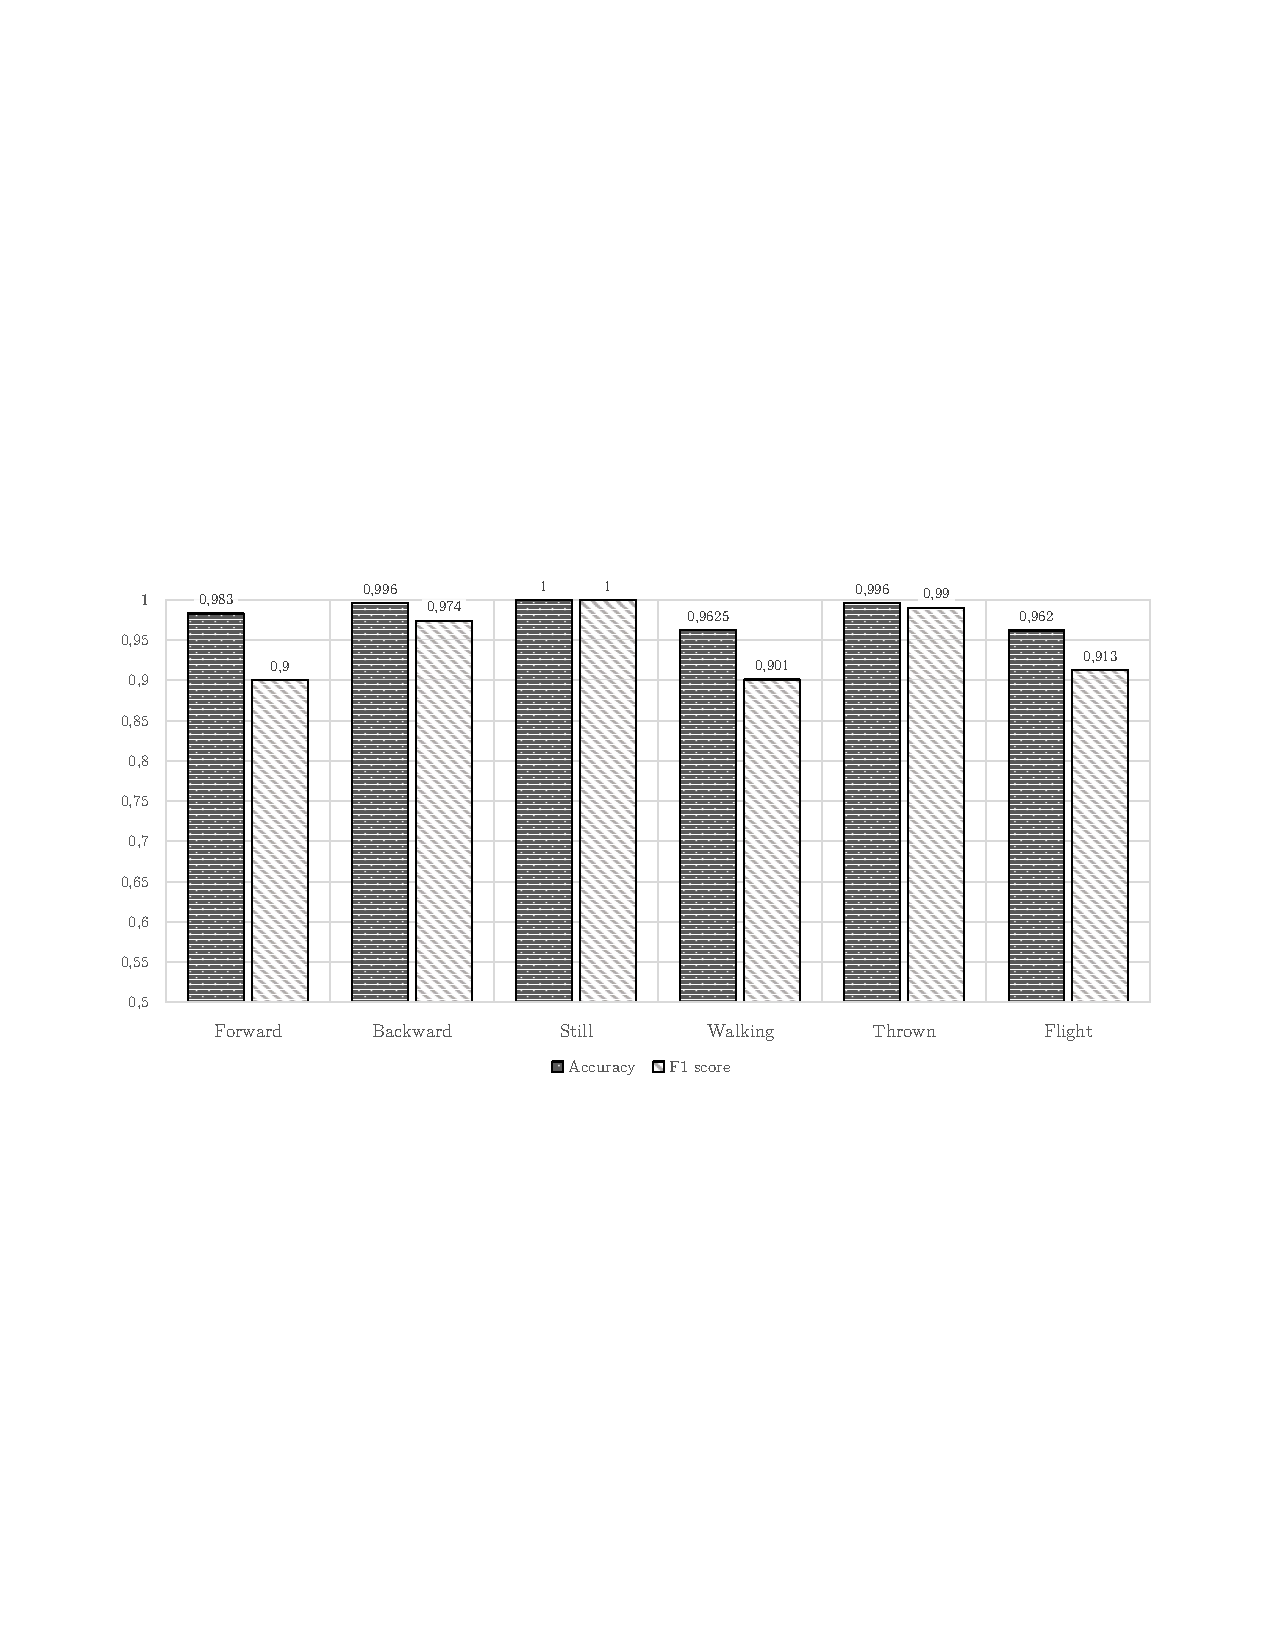
\includegraphics[width=0.8\paperwidth]{img/rnn_results.pdf}}
		\caption{RNN testing results.}
	\end{figure}
\end{center}

\begin{center}
	\begin{figure}[ht!]
		\makebox[\textwidth]{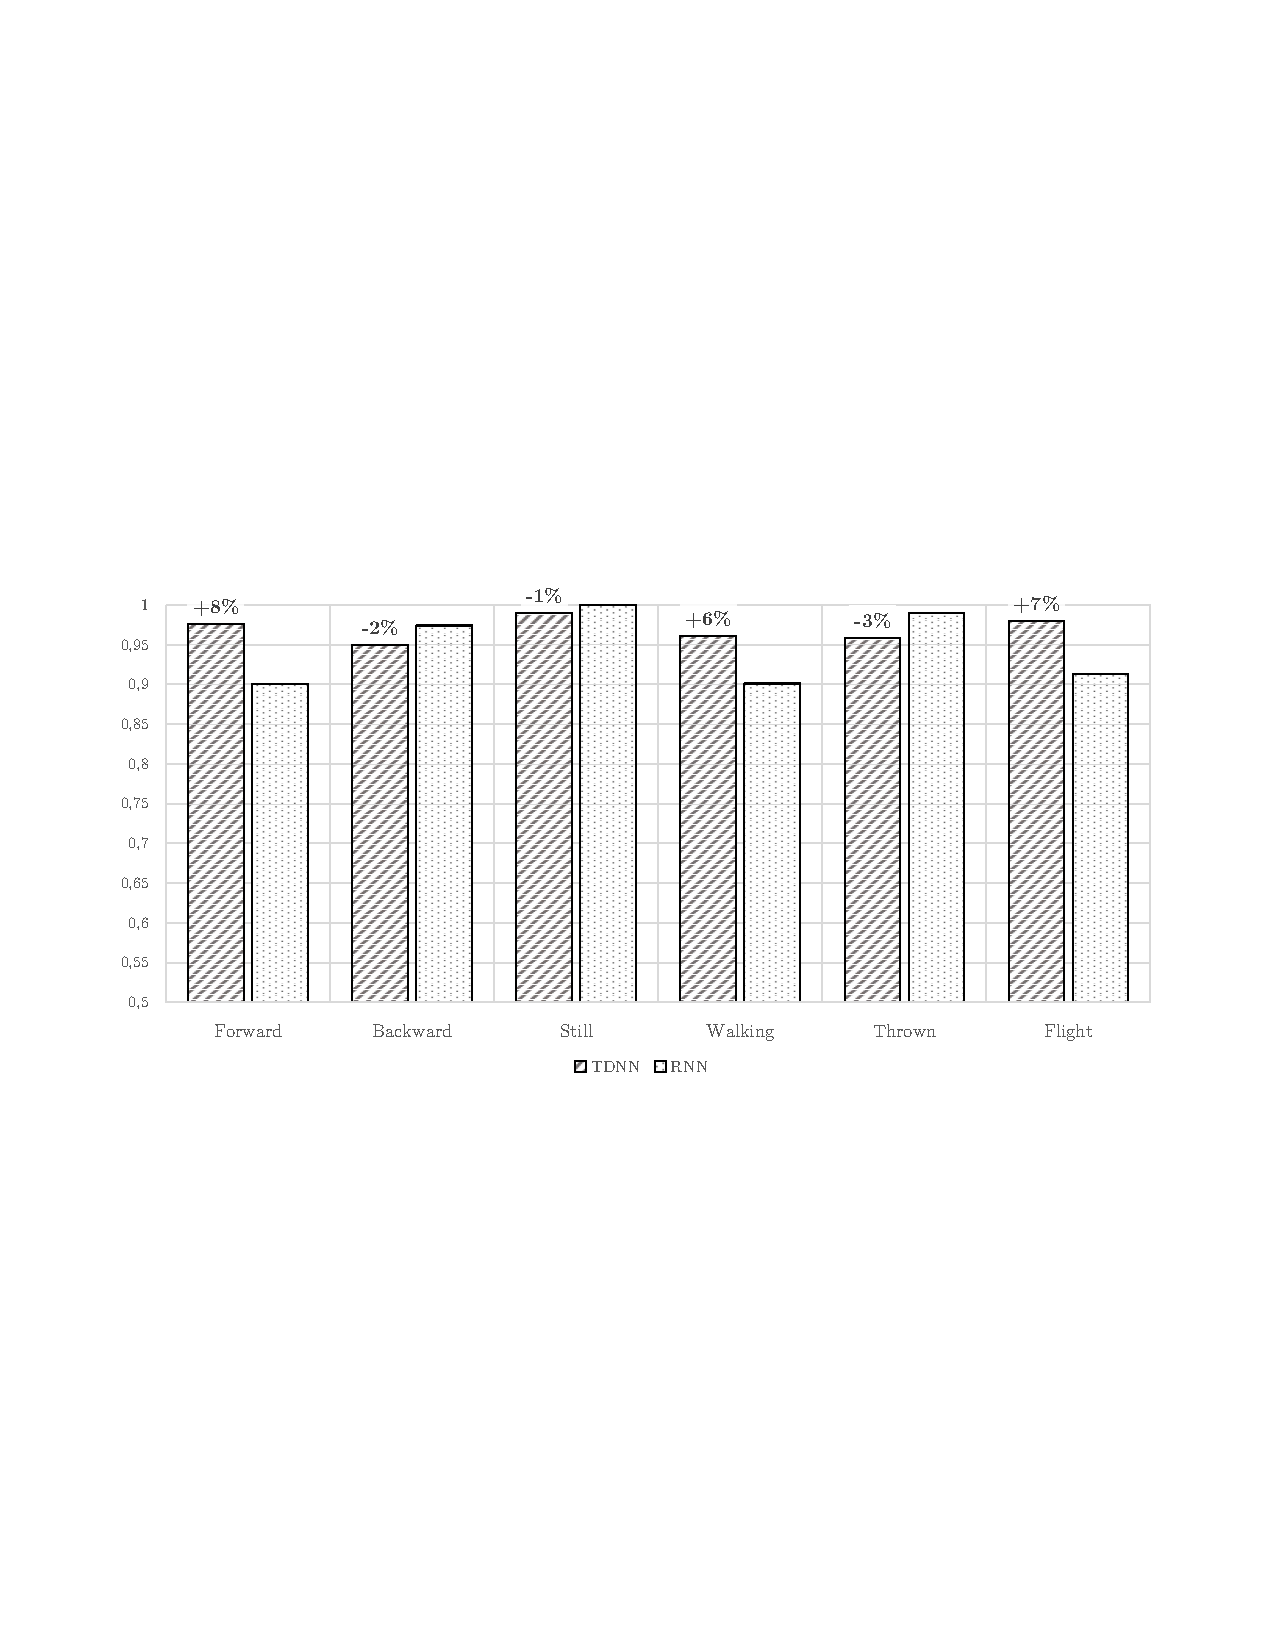
\includegraphics[width=0.8\paperwidth]{img/networks_comparison.pdf}}
		\caption{F1 score comparison between TDNN and RNN.}
	\end{figure}
\end{center}
